\documentclass[11pt,a4paper]{article}
\usepackage[margin=2.1cm,headheight=16pt]{geometry}
\usepackage[T1]{fontenc}
\usepackage{lmodern}
\usepackage{xcolor}
\usepackage{graphicx}
\usepackage{booktabs}
\usepackage{tabularx}
\usepackage{fancyhdr}
\usepackage{float}
\usepackage[hidelinks,colorlinks=true,linkcolor=febblue,urlcolor=febblue]{hyperref}
\definecolor{febblue}{HTML}{1C4687}
\definecolor{febgold}{HTML}{FDB515}
\definecolor{codebg}{HTML}{F3F4F6}
\newcommand{\file}[1]{\texttt{#1}}
\setlength{\parskip}{4pt}
\pagestyle{fancy}
\fancyhf{}
\fancyhead[L]{\color{febblue}\textbf{FEBAUTO Racing}}
\fancyhead[R]{\color{febblue}Hardware options report}
\fancyfoot[C]{\thepage}
\renewcommand{\headrule}{\color{febgold}\hrule width\headwidth height 0.8pt}
\graphicspath{{figs/}}

\begin{document}

\begin{titlepage}
  \centering
  \vspace*{1.5cm}
  
\includegraphics[width=4.5cm]{../../assets/feb_logo_512.png}\\[1.2cm]
  {\color{febblue}\Huge\bfseries Autonomous Racing Hardware}\\[6pt]
  {\Large Options, costs and benefits}\\[1.5cm]
  {\large Formula Electric at Berkeley, Autonomous Team}\\[4pt]
  September 2026\\[2cm]
  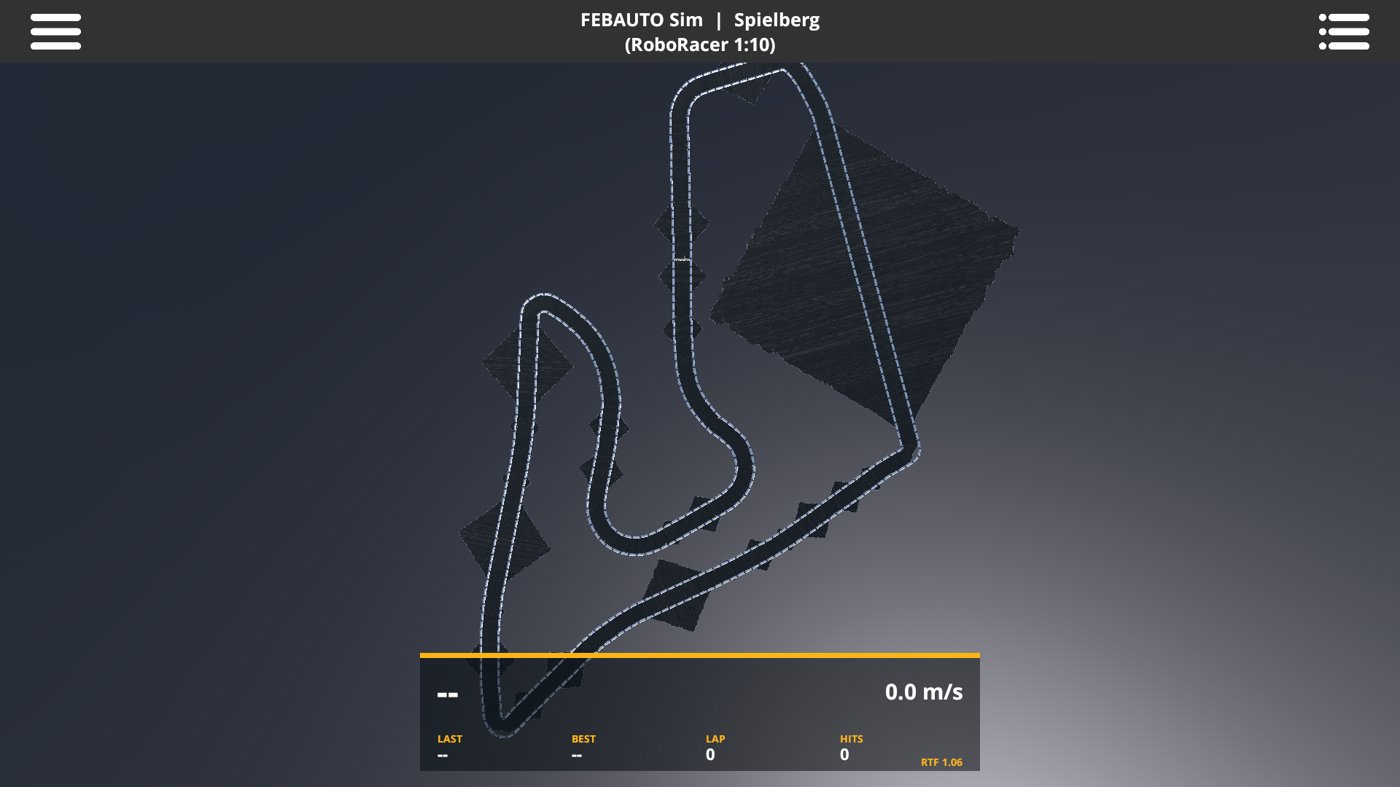
\includegraphics[width=0.8\linewidth]{spiel_track.jpg}\\[6pt]
  {\small The FEBAUTO simulator running the Red Bull Ring (Spielberg) at 1:10 scale.}
\end{titlepage}

\tableofcontents
\newpage

\section{Executive summary}

The autonomous team has built a complete software racing platform in the last month: a
native simulator of the RoboRacer 1:10 race car, a containerised ROS~2 devkit, a starter
driving stack, a competition harness, a leaderboard and two manuals. It onboards a new member
in an hour and runs a full season (qualification, time-attack, head-to-head final) with no
hardware. Its one limit is that the code never meets a real car.

This report lays out six options for closing that gap, from staying software-only to a
1:5-scale vehicle, with a full bill of materials for each, and recommends
\textbf{Plan~B: one RoboRacer-standard 1:10 car with a Hokuyo lidar and a lab track, about
\$3{,}000}, with \textbf{Plan~C, a second car, next semester}. Two options the committee asked
about specifically, converting the team's Tamiya chassis and moving to a 1:4 or 1:5 scale car,
are analysed in sections~\ref{sec:tamiya} and~\ref{sec:large} and found not to be feasible for reasons of
eligibility, community, track size and safety rather than cost. The depth camera the team
already owns is assumed available and is not priced.

\begin{table}[H]
\centering
\begin{tabularx}{\linewidth}{lXrl}
\toprule
Plan & What & Cost (USD) & Verdict \\
\midrule
0 & Simulator only (status quo) & 0 & keep as the base of everything below \\
A & One 1:10 car, budget sensors and compute & 1{,}400 & viable; upgrade path to B \\
\textbf{B} & \textbf{One 1:10 car, RoboRacer reference build} & \textbf{3{,}000} & \textbf{recommended} \\
C & Two 1:10 cars (B + a budget second car) & 4{,}400 & recommended for the following semester \\
D & Convert the team's Tamiya 1:10 chassis & 1{,}200 & not feasible for competition; poor value \\
E & 1:5-scale vehicle & 6{,}500+ & not feasible: track, safety, no community \\
\bottomrule
\end{tabularx}
\caption{The options at a glance. All costs include compute, lidar, power, mounting and the lab track kit; prices are September 2026 list prices, rounded, to be verified at order time.}
\end{table}

\section{What exists today: the FEBAUTO simulator platform}

\begin{figure}[H]
\centering
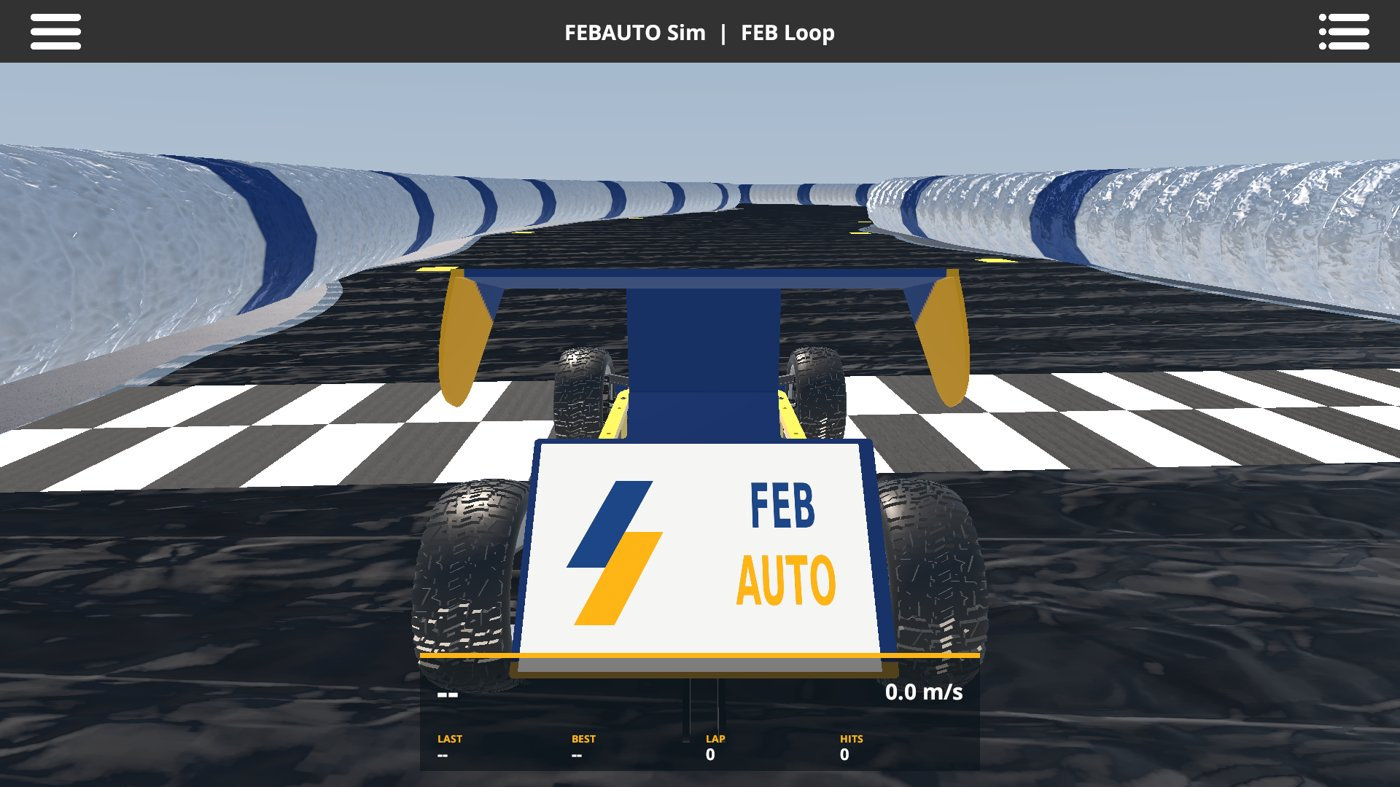
\includegraphics[width=0.49\linewidth]{cam1.jpg}\hfill
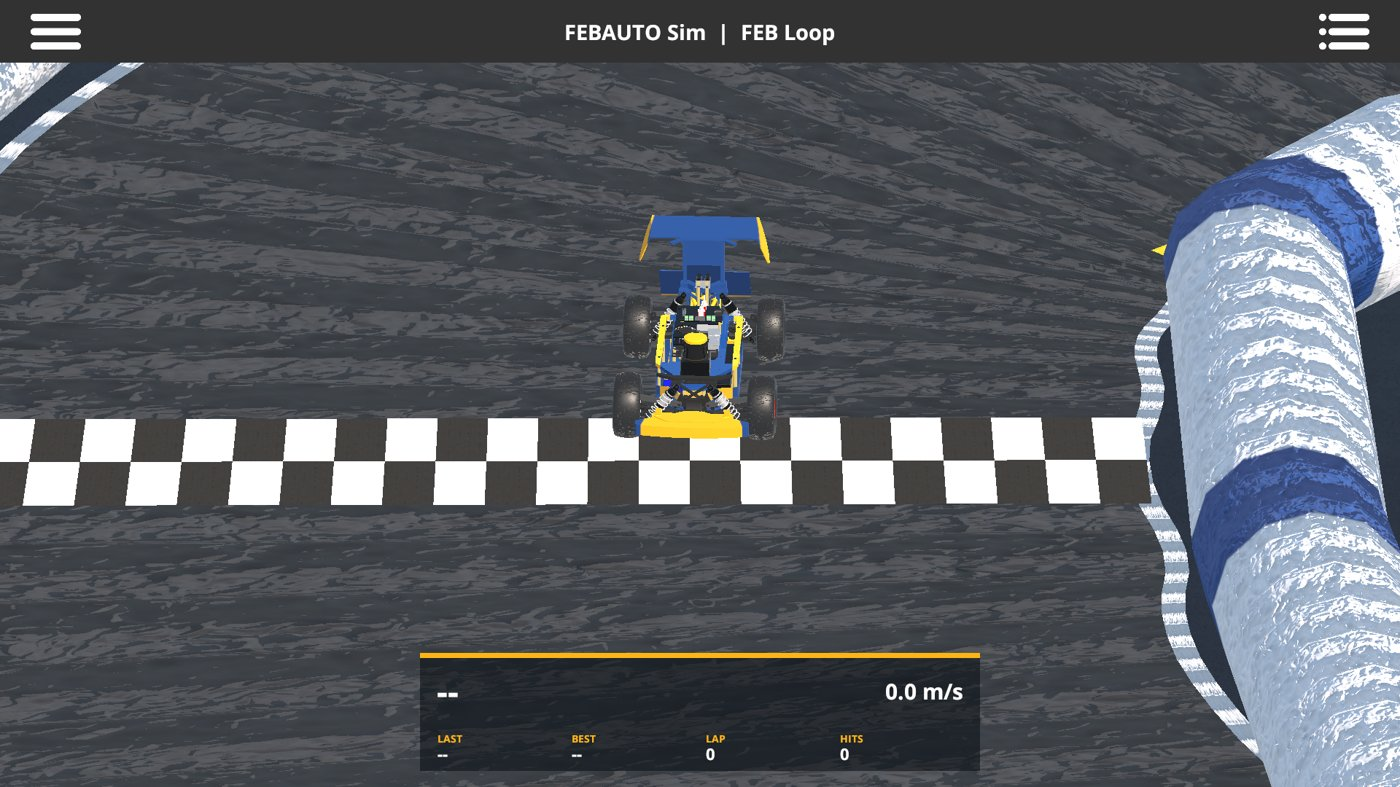
\includegraphics[width=0.49\linewidth]{cam3.jpg}\\[3pt]
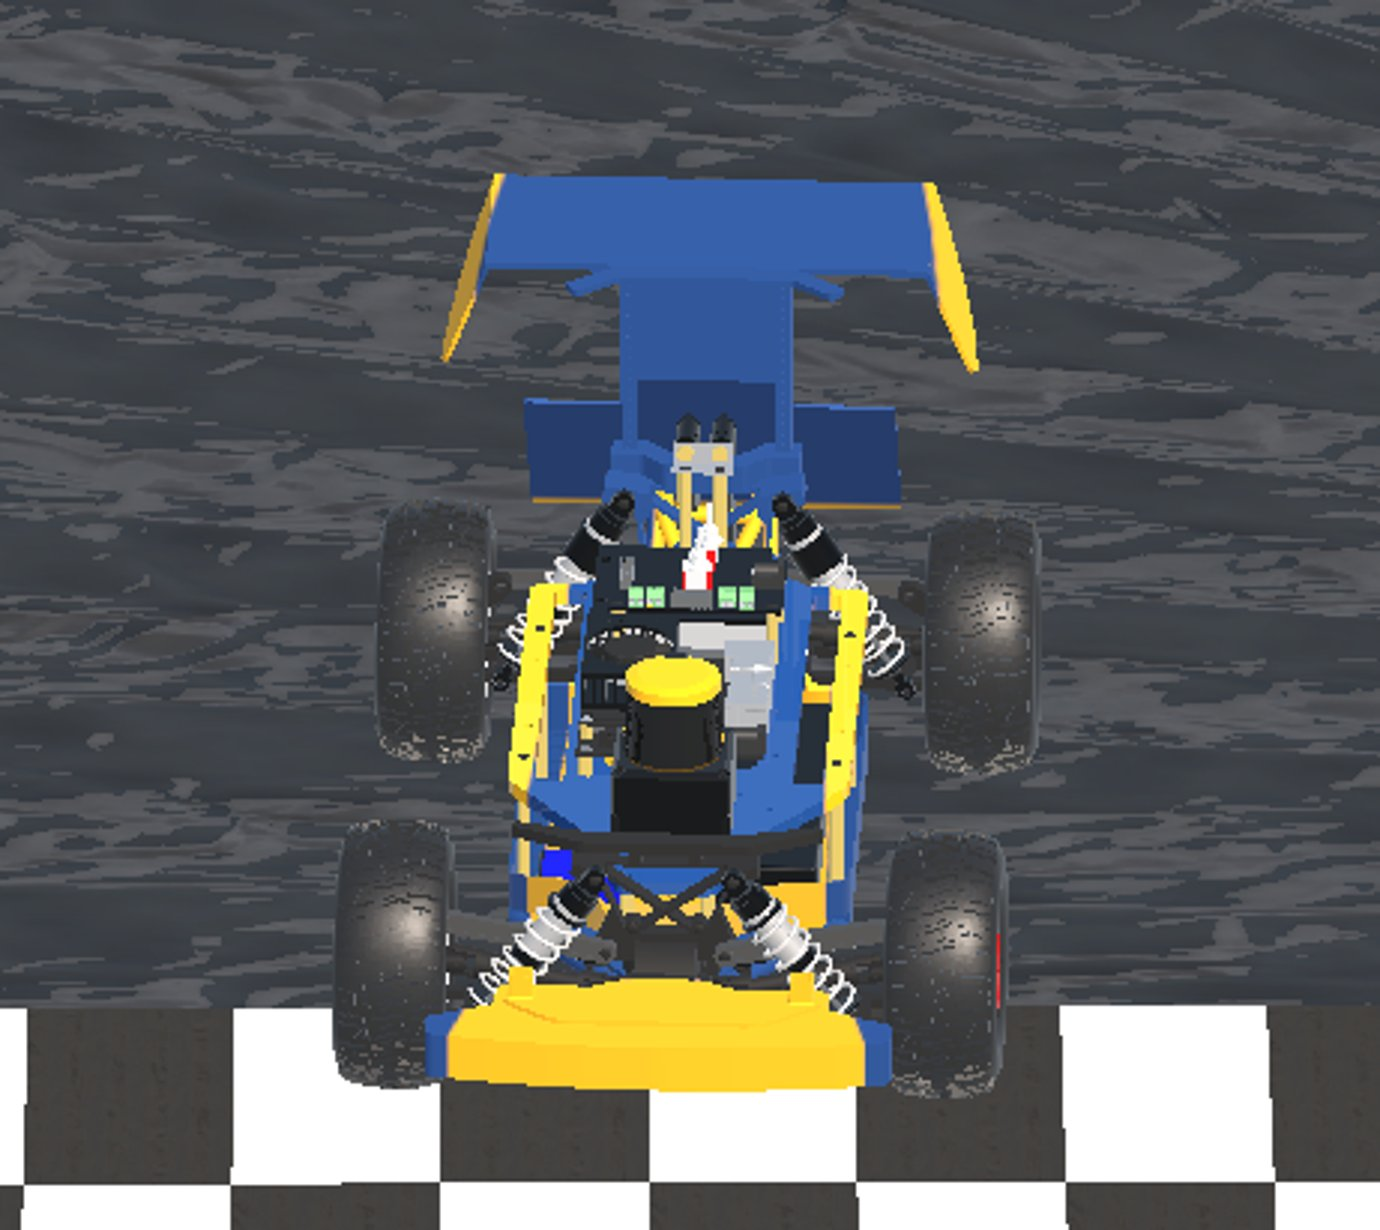
\includegraphics[width=0.49\linewidth]{base_crop3.jpg}\hfill
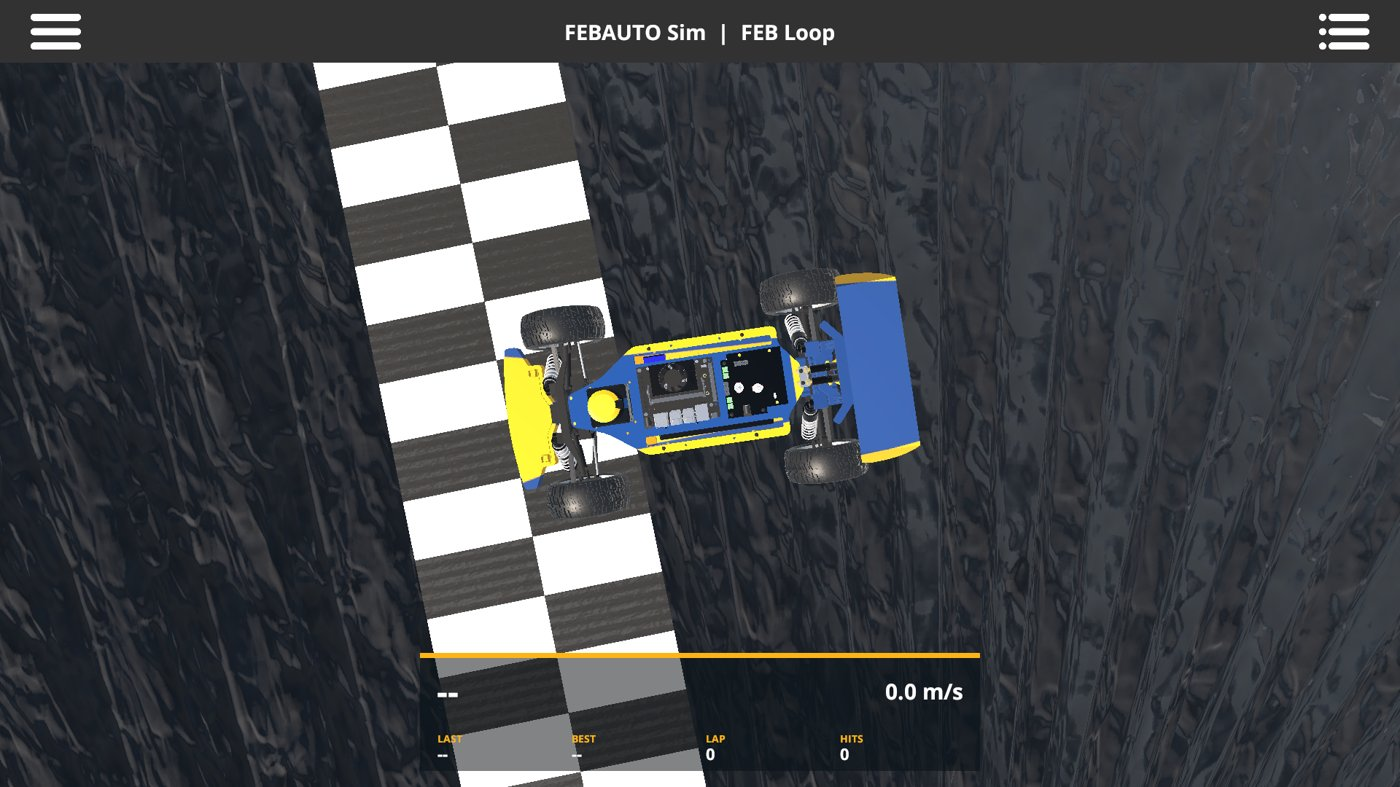
\includegraphics[width=0.49\linewidth]{cam2.jpg}
\caption{The RoboRacer car in the FEBAUTO simulator: chase view with the race HUD, front view, and two overhead views. The vehicle model is the league's digital twin, unchanged; the livery and dressing are cosmetic.}
\end{figure}

\subsection{The platform}

\begin{tabularx}{\linewidth}{lX}
\toprule
Piece & What it does \\
\midrule
Simulator & Native Mac, Windows and Linux app, a fork of the AutoDRIVE simulator. Tracks load from folders at run time (walls of 33~cm air duct, or FSAE-style cones). Up to four cars. Visual and bare looks. Race HUD, ghost lap, real-time factor readout. \\
Devkit & Docker image with ROS~2 Humble and the simulator bridge; the member's code runs inside it; Foxglove for live visualisation on any laptop with nothing else installed. \\
Starter kit & A commented reactive driver that laps any track, tuning file, system-identification tool, and a learning path from tuning to mapping, racelines and model-predictive control. \\
House racer & A conservative opponent car for practising overtakes. Starts only when the member's own stack starts. \\
Harness & Runs every submitted image on a secret track under league rules, records bags, audits banned topics, writes results, seeds and runs knockout brackets. \\
Site & Practice boards per track, qualification progress per team, event standings and brackets. \\
Manuals & Competitor manual (install to leaderboard entry) and organiser manual (tracks, events, race day, releases). \\
\bottomrule
\end{tabularx}

\subsection{Tracks}

Tracks are folders of a PNG and a YAML file, so a new one takes minutes and needs no rebuild.
The team ships four: the FEB Loop, the same loop with FSAE cones instead of walls, the
RoboRacer league's Porto practice track, and a custom circuit with a hairpin, esses and a
chicane. Real circuits from the RoboRacer track database import directly: the Red Bull Ring
at 1:10 scale, 342~m long, is shown on the cover and below.

\begin{figure}[H]
\centering
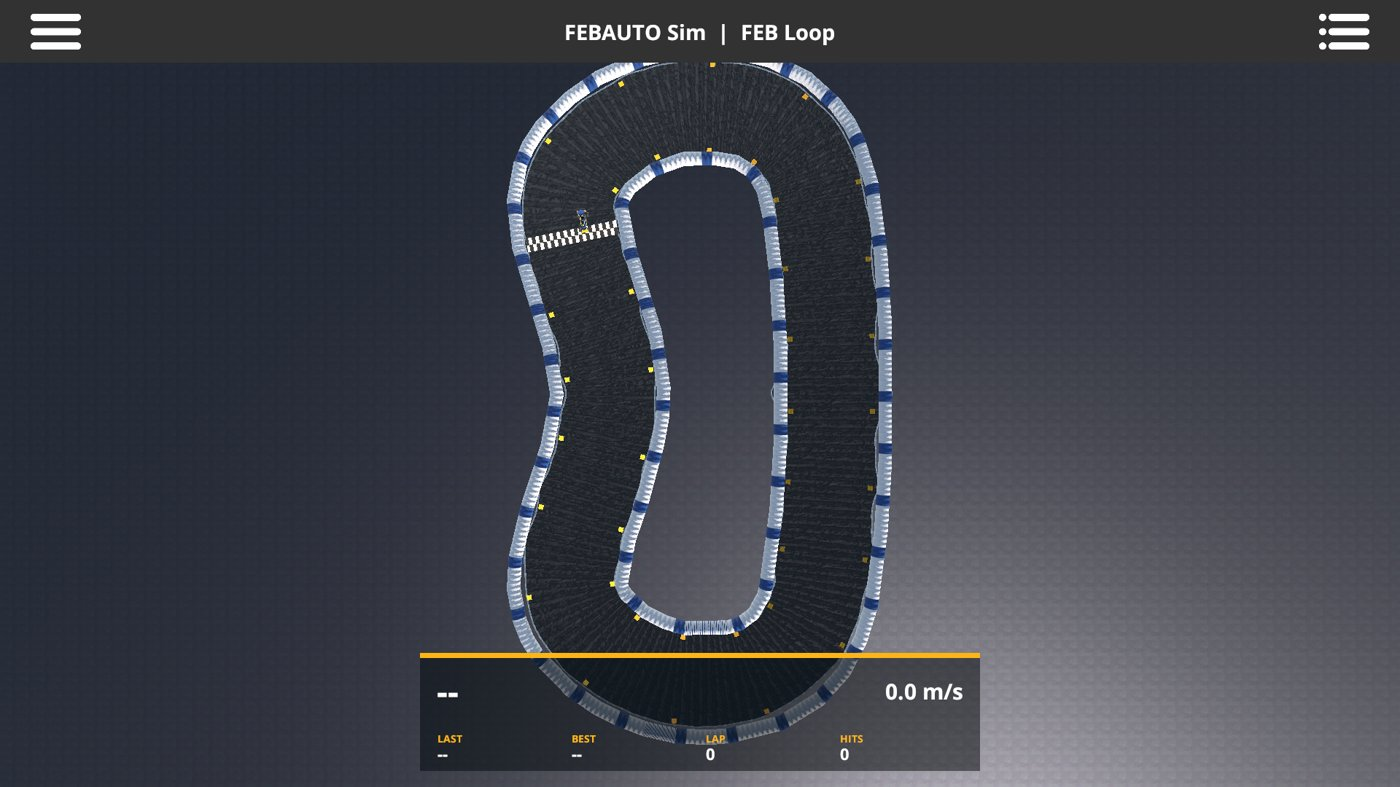
\includegraphics[width=0.32\linewidth]{cam6.jpg}\hfill
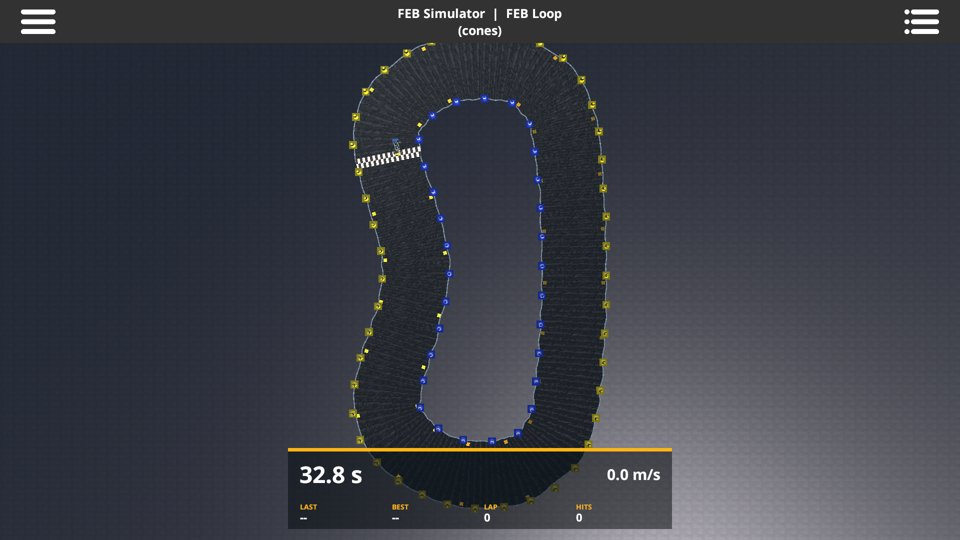
\includegraphics[width=0.32\linewidth]{v_cones.jpg}\hfill
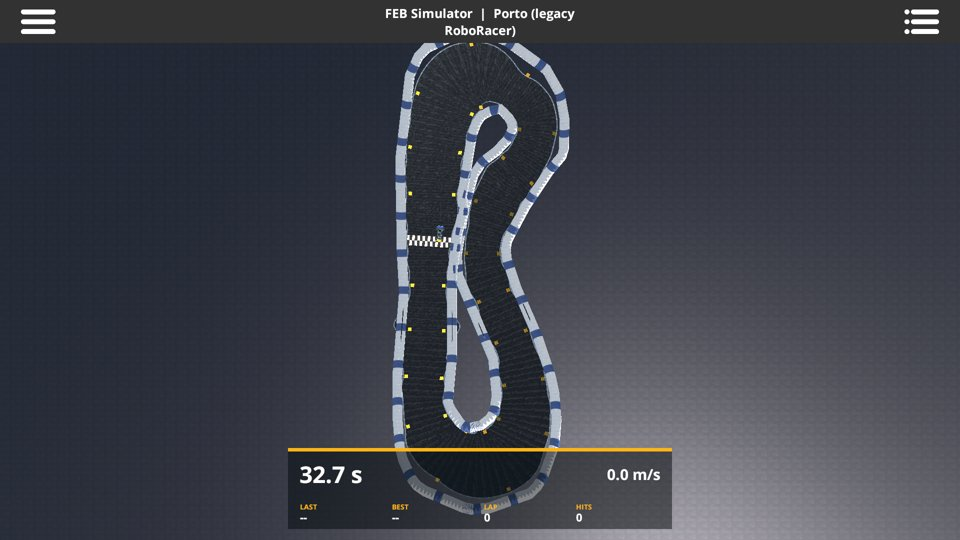
\includegraphics[width=0.32\linewidth]{v_porto.jpg}\\[3pt]
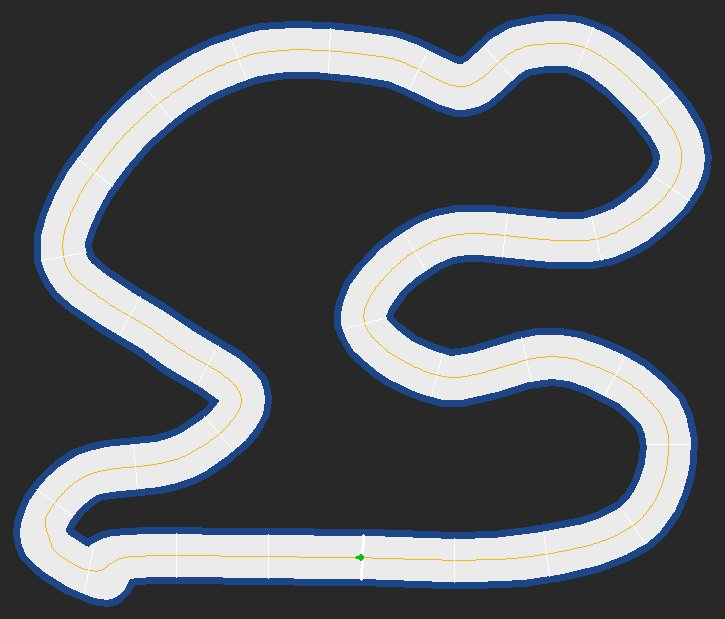
\includegraphics[width=0.49\linewidth]{circuit_preview.jpg}\hfill
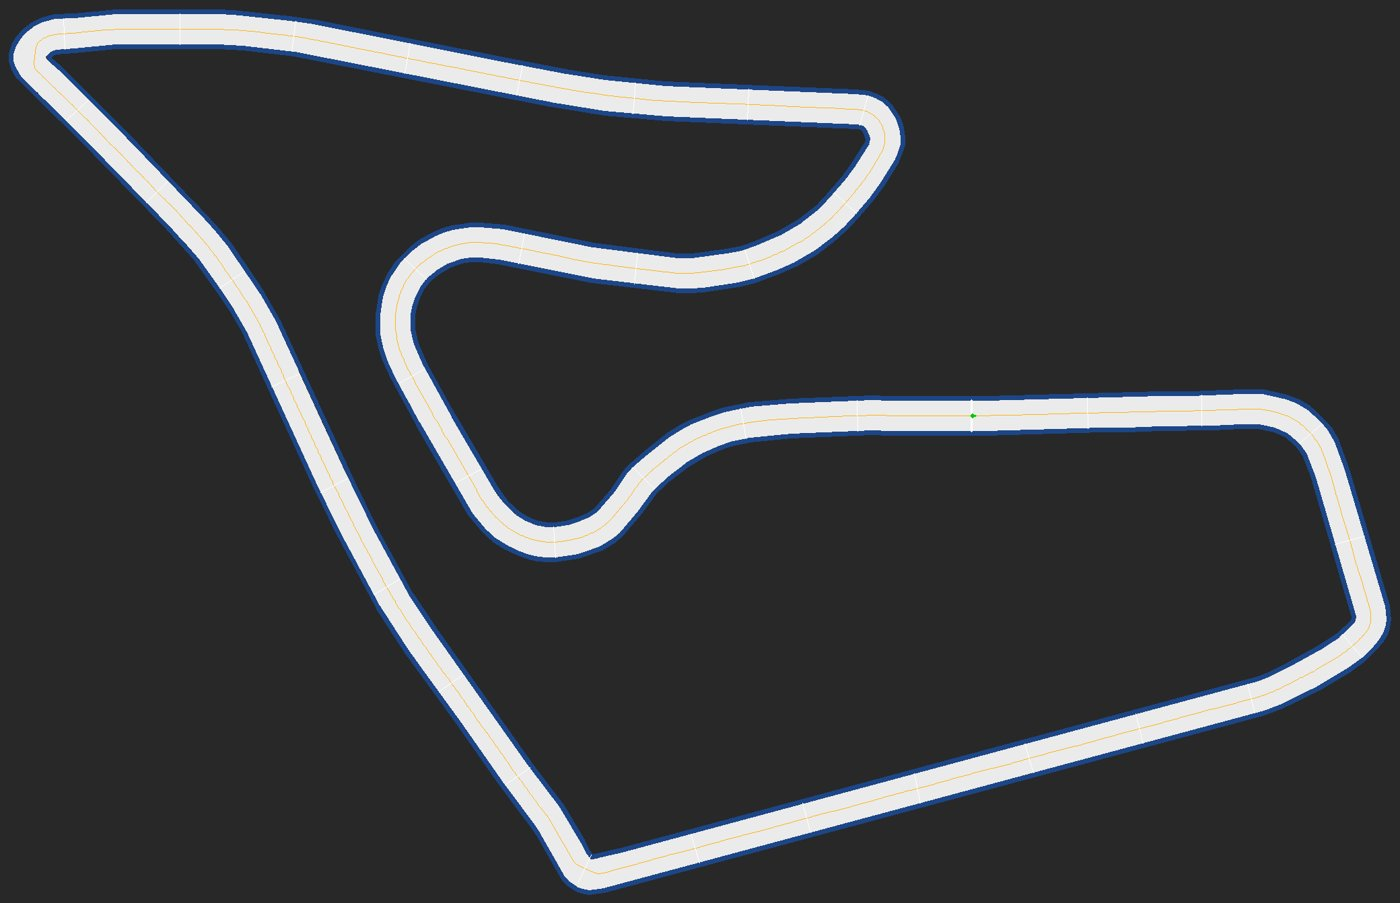
\includegraphics[width=0.49\linewidth]{spielberg_preview.jpg}
\caption{Top: the FEB Loop, its cone version, and Porto, in the simulator. Bottom: the generated maps of the custom FEB Circuit (138~m) and of Spielberg at 1:10 (342~m), with walls, centreline and checkpoints.}
\end{figure}

\subsection{Onboarding and the season}

A new member clones one repository, runs one setup command and drives manually. Copying the
starter kit and running one more command puts an autonomous car on track; the first
leaderboard entry follows the same afternoon. To qualify for the first competition a team
completes ten laps with at most one collision on every practice track. Qualified teams race a
time-attack on a secret track, and the top seeds meet in a two-car knockout final.

\begin{figure}[H]
\centering
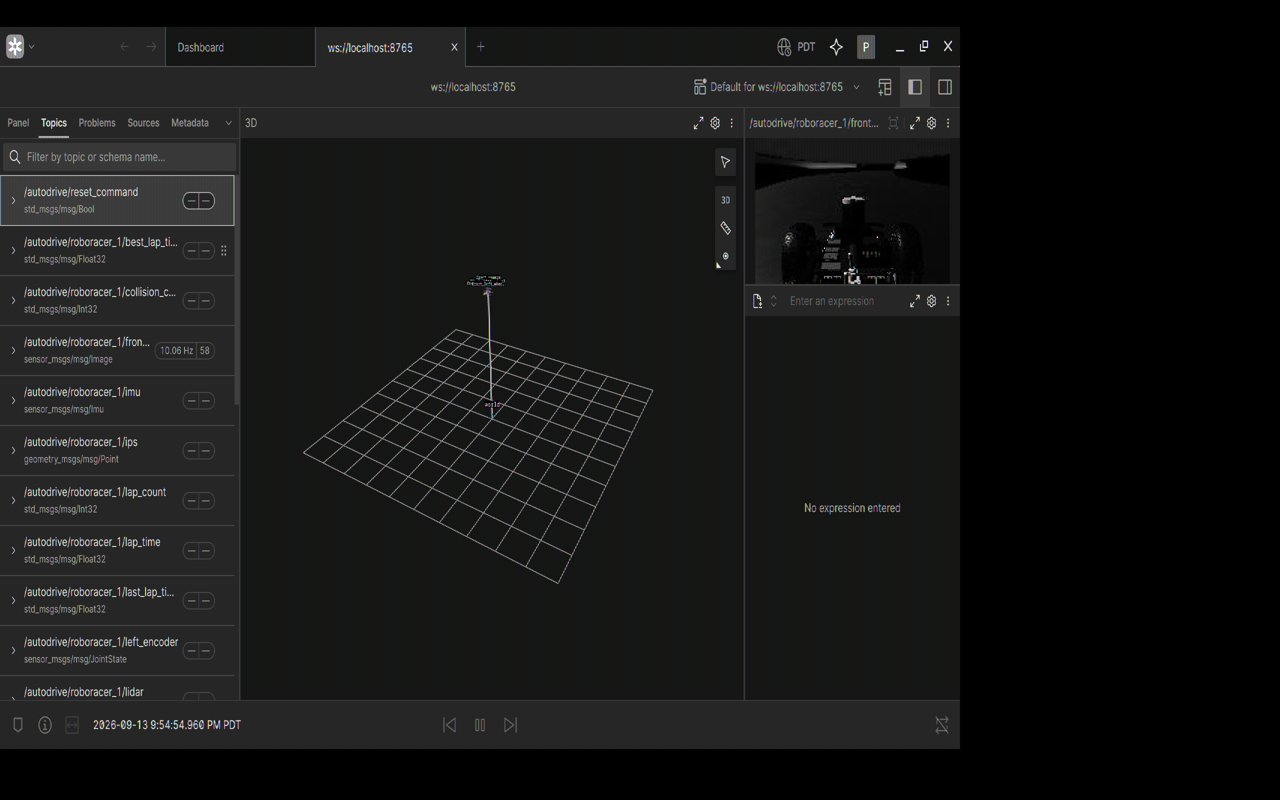
\includegraphics[width=0.49\linewidth]{fox2.jpg}\hfill
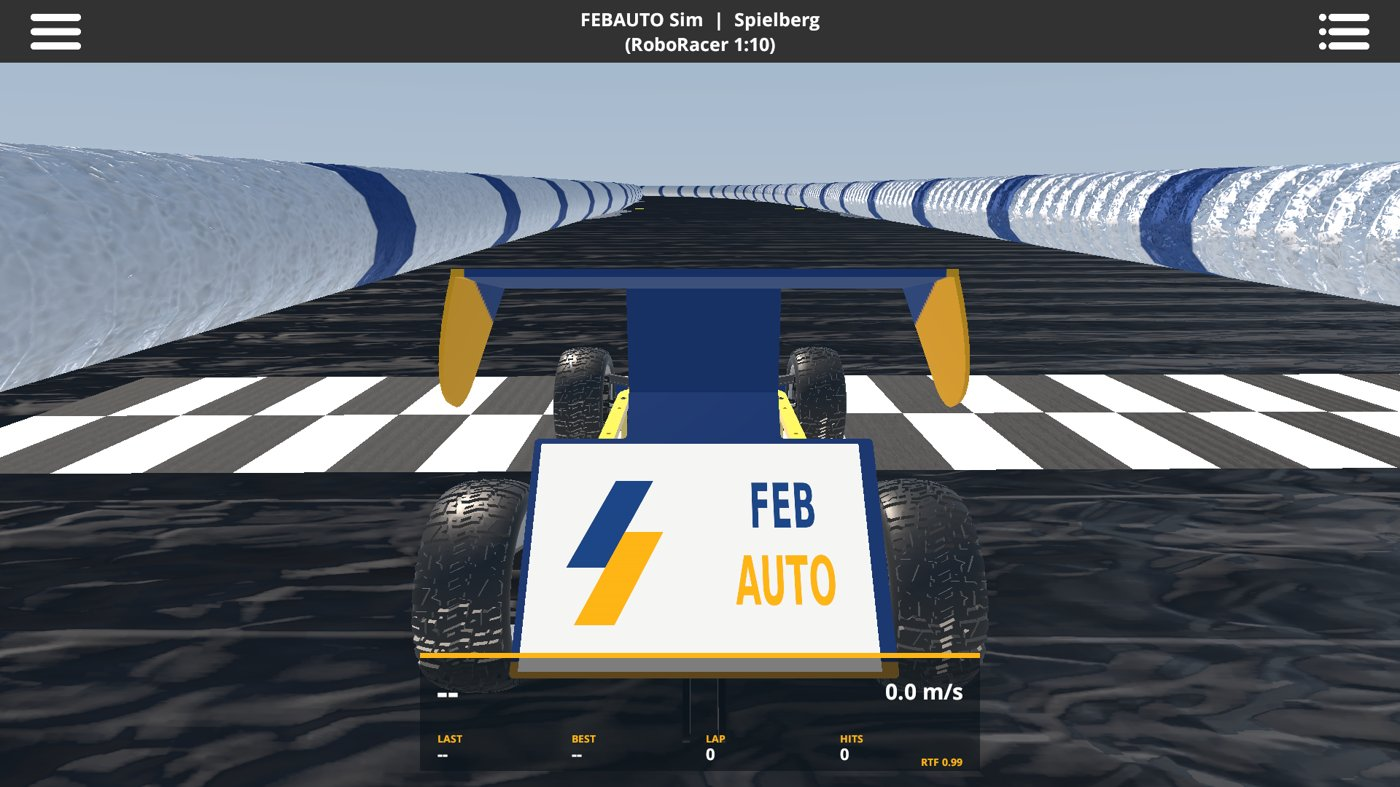
\includegraphics[width=0.49\linewidth]{spiel_driver.jpg}
\caption{Left: Foxglove connected to the devkit, showing the car's topics and the front camera live. Right: the driver's view on Spielberg.}
\end{figure}

\section{Why hardware, and why in the off-season}
\label{sec:why}

The FSAE car is not ready for autonomous work for most of the year: it is being designed,
built, or raced by the rest of the team, and it is never available for an untested stack.
A 1:10 car fills exactly that gap.

\begin{itemize}
  \item \textbf{Sim-to-real is the point of the exercise.} The simulator's car is the digital twin of the RoboRacer reference vehicle. A stack tuned in the simulator is meant to transfer; without a car the claim is never tested, and members never meet real latency, tyre variation, a lidar that sees the room, or a battery that sags.
  \item \textbf{Off-season continuity.} Perception, localisation, planning and control are the same problems at 1:10 and at full scale. The 1:10 car is where the team develops and validates them between seasons, on a table in the lab, without waiting for the FSAE vehicle or a test day.
  \item \textbf{Driverless FSAE readiness.} Formula Student driverless events use cone tracks and camera plus lidar perception. The cone version of every FEBAUTO track exists for this reason; a real car with a camera and a 2D lidar lets the team practise that exact pipeline at small scale.
  \item \textbf{Competitions and recruiting.} RoboRacer runs physical races at ICRA, IROS and IFAC every year on the rules our league already uses. A car on a table is also what keeps a room full of new members after the first semester.
  \item \textbf{Cost of not doing it.} The software platform is done and free to run. Its value compounds only if what members build on it reaches hardware.
\end{itemize}

\section{The options}

Every plan includes compute, lidar, power, mounting and the track kit of section~\ref{sec:track}.
Where a part is available in more than one grade, the table names the one priced.

\subsection{Plan 0: simulator only}

Cost \$0. Everything in section~2 continues. No sim-to-real work, no physical competition,
no perception on real sensors. Kept as the base layer of every other plan, not as an answer on
its own.

\subsection{Plan A: one 1:10 car, budget grade}

\begin{tabularx}{\linewidth}{p{6.2cm}rX}
\toprule
Item & USD & Note \\
\midrule
Traxxas Slash 4x4 VXL (TRA68086) & 500 & the RoboRacer-eligible chassis; includes brushless motor and stock ESC \\
VESC-compatible controller, Flipsky mini (75100 or 6.7) & 130 & replaces the stock ESC; wheel odometry and IMU \\
Compute: Raspberry Pi 5, 8~GB, cooler, SD card & 120 & enough for lidar-only reactive driving and ROS~2 \\
2D lidar: Slamtec RPLidar A2M12 & 320 & 12~m, 12~Hz, 0.25\textdegree; competition-legal \\
Two 3S 5000~mAh LiPo, charger, safety bag & 190 & \\
Power: buck converter, XT60 splitter, fuse & 30 & instead of the RoboRacer powerboard \\
Plates, standoffs, fasteners, USB hub, cables & 90 & plates laser-cut on campus from the published drawings \\
Spares: tyres, pinion, bumper & 60 & \\
Track kit (section~\ref{sec:track}) & 240 & \\
\midrule
\textbf{Total} & \textbf{1{,}680} & about \$1{,}400 without the track kit \\
\bottomrule
\end{tabularx}

\medskip
\textbf{Benefits:} the cheapest real car that runs the same ROS~2 stack as the simulator and
is eligible for RoboRacer events. \textbf{Limits:} the Pi cannot run camera perception at
useful rates and the lidar's 12~Hz and range noise cap safe speed at roughly 3~m/s. Both are
upgrades, not rebuilds: swap the compute and lidar and Plan~A becomes Plan~B.

\subsection{Plan B: one 1:10 car, RoboRacer reference build (recommended)}

\begin{tabularx}{\linewidth}{p{6.2cm}rX}
\toprule
Item & USD & Note \\
\midrule
Traxxas Slash 4x4 VXL (TRA68086) & 500 & chassis with brushless motor \\
VESC 6 MkVI & 260 & the reference controller \\
Compute: NVIDIA Jetson Orin Nano developer kit & 250 & camera perception and learning-based stacks \\
2D lidar: Hokuyo UST-10LX & 1{,}500 & the reference sensor; 40~Hz, 270\textdegree, 10~m, the same as the simulator's \\
Two 3S 5000~mAh LiPo, charger, safety bag & 190 & \\
RoboRacer powerboard & 100 & clean rails for Jetson, lidar and VESC; safe shutdown \\
Plates, standoffs, fasteners, USB hub, cables & 90 & \\
Spares: tyres, pinion, bumper & 60 & \\
Depth camera & 0 & the team's Intel RealSense, already owned \\
Track kit (section~\ref{sec:track}) & 240 & \\
\midrule
\textbf{Total} & \textbf{3{,}190} & about \$2{,}950 without the track kit \\
\bottomrule
\end{tabularx}

\medskip
\textbf{Benefits:} the exact car the league, the build guide and our simulator model; camera
plus lidar fusion is possible on day one; nothing to upgrade later. \textbf{Limits:} the lidar
is half the cost and the most fragile part; a bumper and a speed limit for new stacks are
part of the plan.

\subsection{Plan C: two cars}

Plan~B plus a second car built to Plan~A's grade (\$1{,}400, no second track kit): total
about \$4{,}600, or \$4{,}400 if the second car reuses the first car's charger and spares.
\textbf{Benefits:} the head-to-head final on real cars, a spare during a competition, and two
members' stacks testable at once. The budget car is the natural second car because racecraft,
not sensor grade, is what head-to-head tests. Recommended for the semester after Plan~B.

\subsection{Plan D: convert the team's Tamiya 1:10 chassis}
\label{sec:tamiya}

The team owns a motorless Tamiya touring-car chassis. Priced as a full conversion:

\begin{tabularx}{\linewidth}{p{6.2cm}rX}
\toprule
Item & USD & Note \\
\midrule
Tamiya chassis & 0 & owned \\
Brushless motor and ESC or VESC, steering servo & 200 & the kit has neither \\
Compute, lidar, power, cables as Plan~A & 760 & \\
Custom sensor deck and mounts (design, prints, iterations) & 80 & no published drawings exist for this chassis \\
Track kit & 240 & \\
\midrule
\textbf{Total} & \textbf{1{,}280} & saves about \$400 against Plan~A \\
\bottomrule
\end{tabularx}

\medskip
\textbf{Why it is not feasible as the team's car:}
\begin{itemize}
  \item \textbf{Not competition-eligible.} RoboRacer rules require a Traxxas 1:10 chassis (codes TRA74054, TRA6804R, TRA68086). A Tamiya cannot enter any physical event.
  \item \textbf{Not the simulated car.} Wheelbase, track width, tyre model and steering geometry differ from the digital twin, so simulator tuning does not transfer, which removes the main reason to have a car.
  \item \textbf{No community.} Every RoboRacer document, drawing, VESC profile and forum answer assumes the Slash. On the Tamiya the team solves mounting, power and drivetrain questions alone. That is a semester of mechanical work that teaches no autonomy.
  \item \textbf{Weak platform.} A touring car has 5~mm of ground clearance and no room for a lidar, a computer and a battery. The Slash was chosen by the community because it carries them.
\end{itemize}
The chassis is still useful as a bench mule for wiring and sensor mounting practice, at no cost.

\subsection{Plan E: a 1:5-scale vehicle}
\label{sec:large}

The committee asked about a 1:4 car. No manufacturer makes a 1:4 road car; the nearest
production platforms are 1:5 short-course trucks (Losi 5IVE-T, Arrma Kraton 8S) and 1:6
monster trucks (Traxxas X-Maxx). Priced with the same sensors and compute as Plan~B:

\begin{tabularx}{\linewidth}{p{6.2cm}rX}
\toprule
Item & USD & Note \\
\midrule
1:5 electric chassis (8S class) & 1{,}300 to 1{,}900 & 8 to 12~kg, 50~km/h and up \\
8S battery pair and charger & 500 & \\
High-current controller (VESC 75V/300A class) & 350 & \\
Compute, lidar, camera mount as Plan~B & 1{,}850 & \\
Custom deck, roll protection, kill switch & 400 & nothing published to copy \\
Track: outdoor-sized (see below) & 2{,}000+ & \\
\midrule
\textbf{Total} & \textbf{6{,}400 to 7{,}000} & \\
\bottomrule
\end{tabularx}

\medskip
\textbf{Why it is not feasible:}
\begin{itemize}
  \item \textbf{Track size.} A corridor for a 1:5 car is at least 3~m wide and a lap needs 150~m or more: a parking lot, not a lab. Air-duct walls do not work at that scale; the walls become barriers and the track cannot be stored.
  \item \textbf{Safety.} A 10~kg vehicle at 50~km/h carries about 1~kJ of kinetic energy, thirty times a 1:10 car. It cannot be run indoors, near people, or by a first-semester member's untested stack. It needs a kill switch, roll protection and a marshal.
  \item \textbf{No community and no competition.} No autonomous racing series exists at that scale. Every problem, from mounts to motor control, is solved alone.
  \item \textbf{Not the simulated car.} Nothing built in the simulator transfers.
  \item \textbf{Cost.} Twice Plan~B before the track, and the track is a separate project.
\end{itemize}

\section{The track kit}
\label{sec:track}

\begin{tabularx}{\linewidth}{p{6.2cm}rX}
\toprule
Item & USD & Note \\
\midrule
Flexible aluminium duct, 12--13~inch (33~cm) diameter, 4 lengths of 25~ft (about 30~m total) & 130 & the league's walls; folds flat to store; joins with tape \\
FSAE-style cones, 3D-printed at 1:10 (100 pieces) & 15 & 32~mm tall, blue and yellow filament, about 10~g each; printed on the team's printers \\
Floor tape, start-line gate (photo interrupter), storage tub & 95 & \\
\midrule
\textbf{Total} & \textbf{240} & \\
\bottomrule
\end{tabularx}

\medskip
Thirty metres of duct builds a 12~m by 6~m loop with a hairpin, the same geometry as the FEB
Loop in the simulator. The cones give the cone version of the same track for camera work, and
scale exactly like the simulator's cone tracks.

\section{Sensor fusion and the driverless connection}

The team already owns an Intel RealSense depth camera. With a 2D lidar it gives the sensor pair
used by Formula Student driverless cars at small scale: the camera classifies cones by colour
and the lidar gives precise range and bearing; fusing them yields a cone map, then a track
boundary, then a raceline. The FEBAUTO simulator publishes both a front camera image and a
lidar scan on the same topics the real car will use, and its cone tracks exist for exactly
this pipeline. Plans~B and~C support this on day one; Plan~A's compute is enough for lidar-only
driving and can be upgraded to a Jetson for camera work later.

\section{Racing: one on one}

The head-to-head final is the season's finish. In the simulator two cars race on one track,
each team's stack in its own container, contact costs both cars a penalty and a respawn, and
the finishing order is laps then time. The figures below are a race on Spielberg between the
starter kit and the house racer.

\begin{figure}[H]
\centering
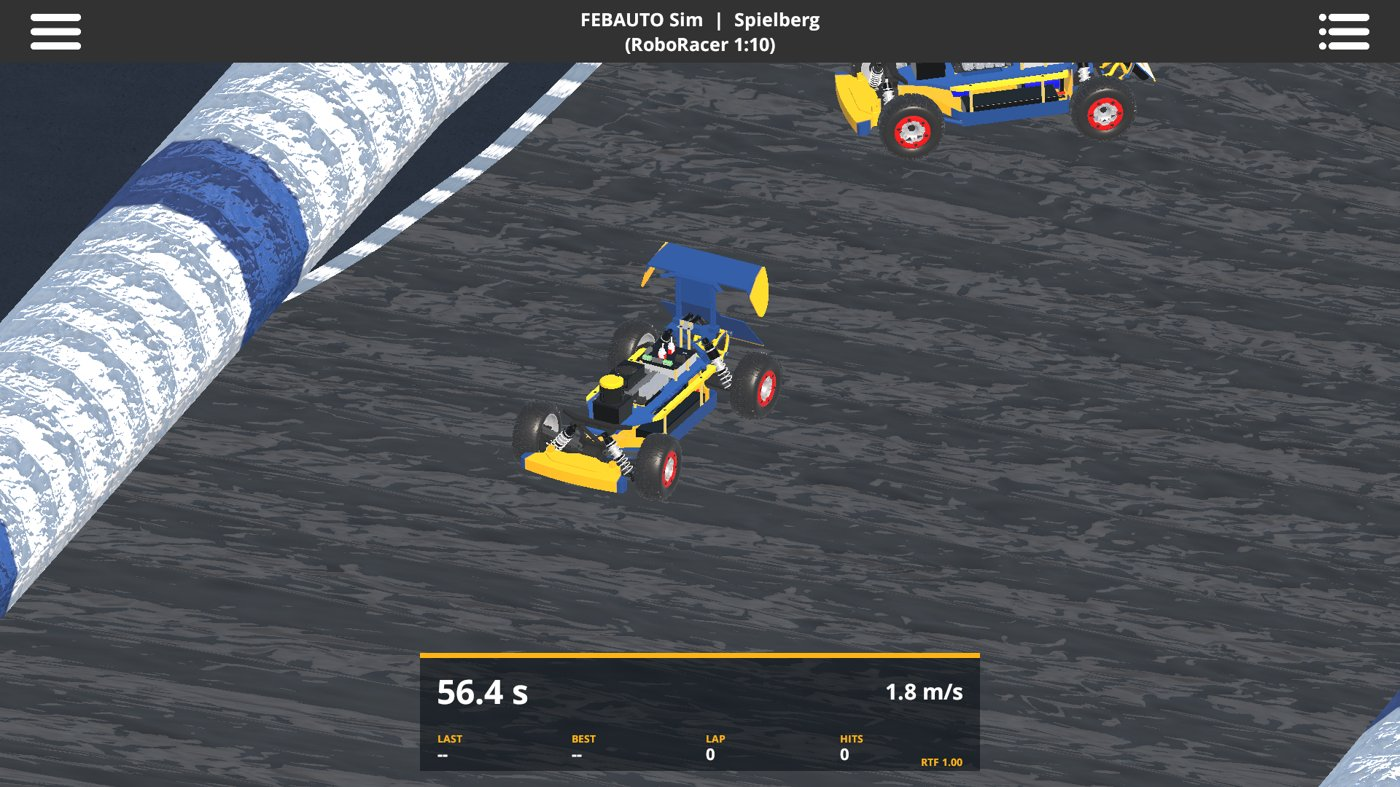
\includegraphics[width=0.49\linewidth]{srace_a.jpg}\hfill
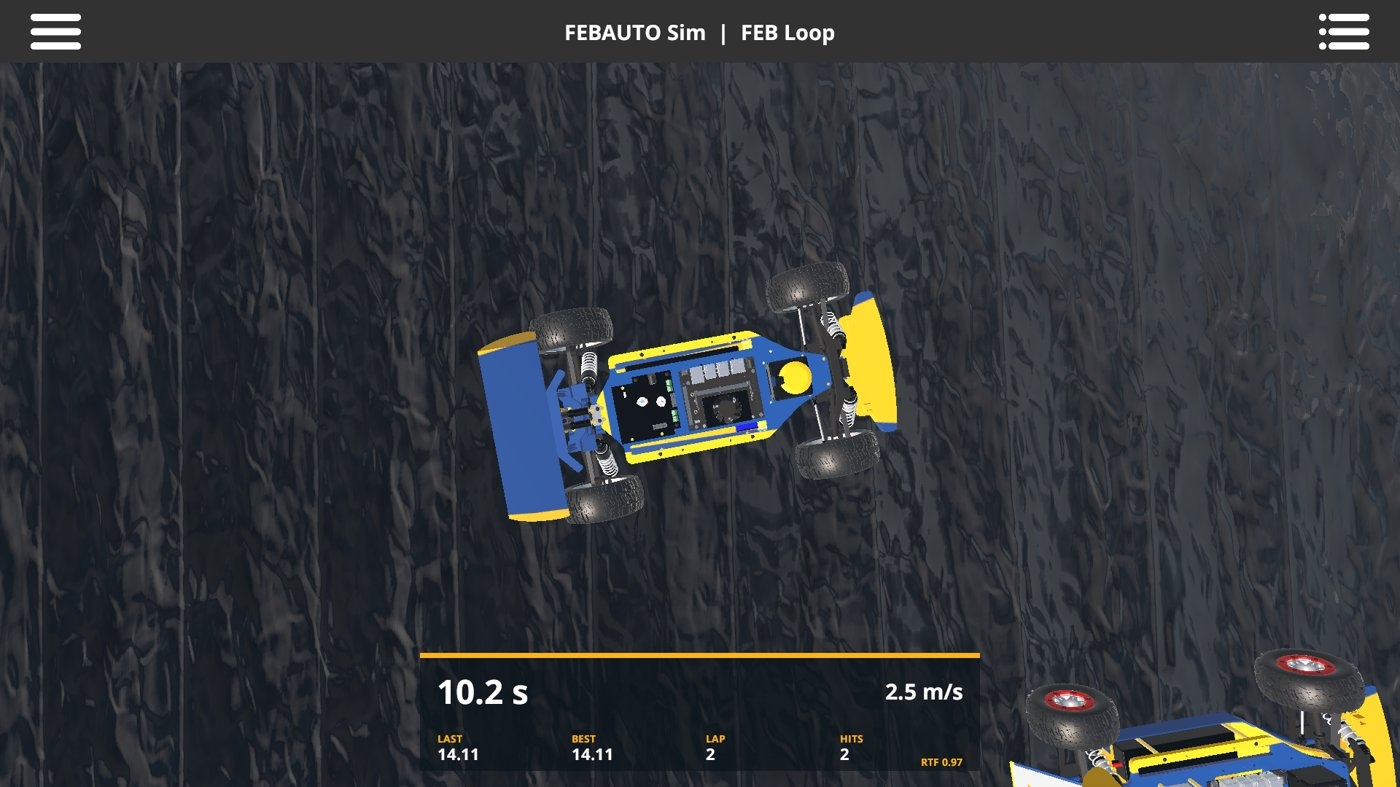
\includegraphics[width=0.49\linewidth]{srace_b.jpg}\\[3pt]
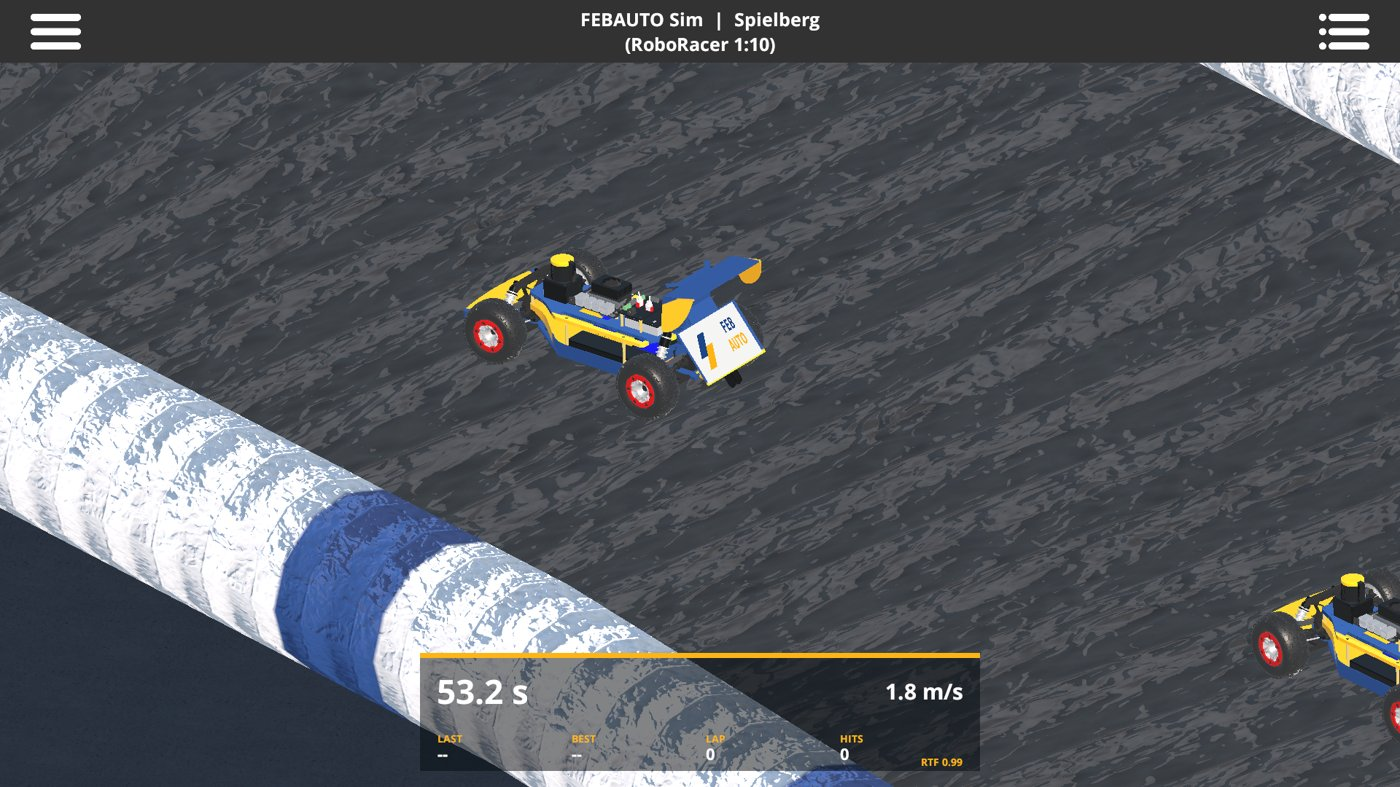
\includegraphics[width=0.49\linewidth]{srace_c.jpg}\hfill
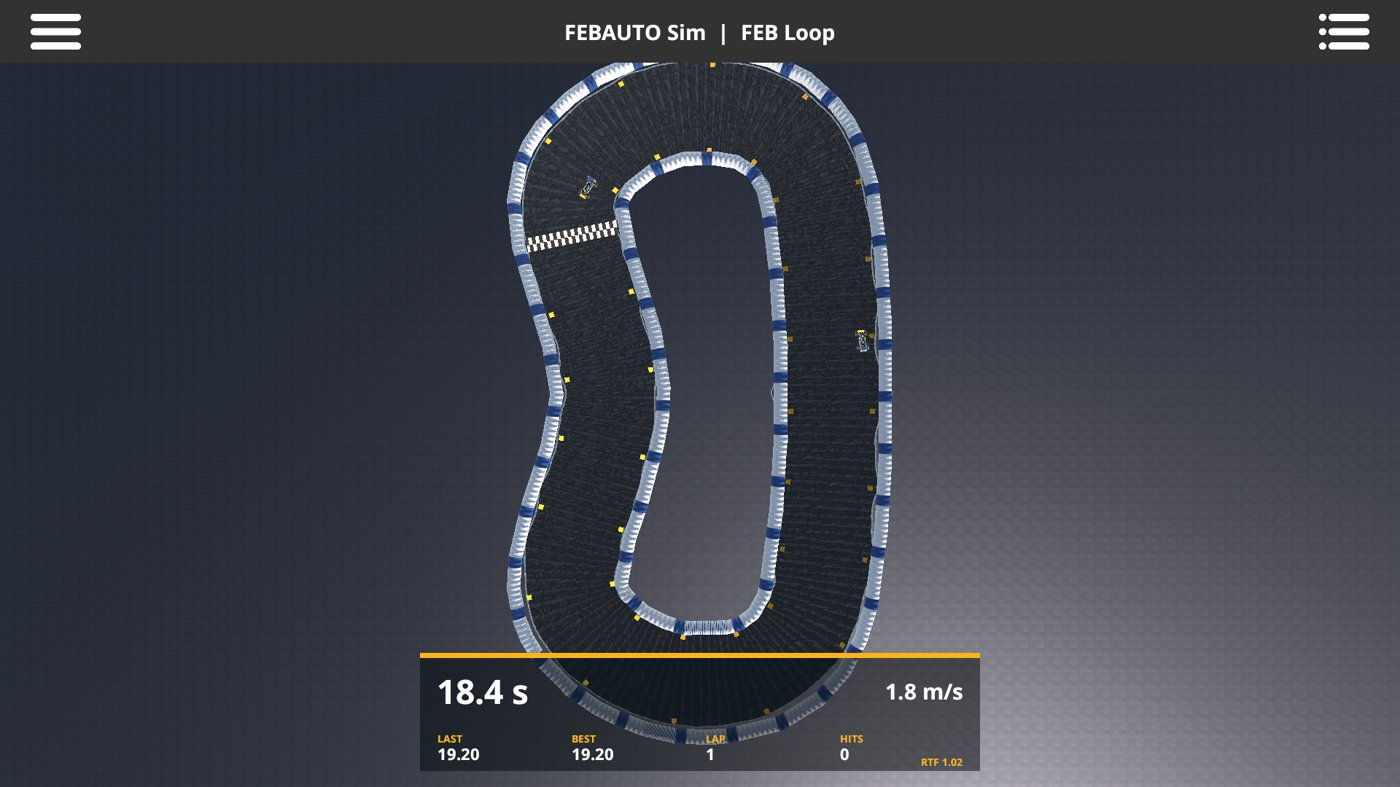
\includegraphics[width=0.49\linewidth]{srace_d.jpg}
\caption{One-on-one AI racing. Top: on Spielberg, the house racer (top of frame, left) closing on the member's car, and a moment earlier as it enters the frame (right). Bottom: on the FEB Loop, both cars in the same corner from above (left) and the whole track with both cars (right). Each car runs an unchanged competitor image behind the harness proxy; contact costs both cars a penalty and a respawn.}
\end{figure}

With Plan~C the same race runs on two real cars on the lab track.

\section{Recommendation and timeline}

Fund Plan~B now (\$3{,}190 plus 10\,\% contingency, \$3{,}500) and Plan~C's second car next
semester (\$1{,}400). Order the lidar first; its lead time is the longest.

\begin{tabularx}{\linewidth}{lX}
\toprule
When & Milestone \\
\midrule
Order + 2 weeks & Car assembled from the RoboRacer build guide; manual drive; sensors on ROS~2; track laid \\
+ 4 weeks & Starter kit laps the lab track; simulator-to-car gap measured and written up \\
+ 8 weeks & Qualified teams run their stacks on the car; first internal physical time-attack \\
Following semester & Second car; head-to-head on hardware; entry to a RoboRacer physical event \\
\bottomrule
\end{tabularx}

\section{Risks}

\begin{itemize}
  \item \textbf{Crashes.} Bumper, soft duct walls, a speed limit for new stacks; spares budgeted. The lidar is the fragile part and sits behind the bumper line.
  \item \textbf{Batteries.} LiPo bag, supervised charging, a written procedure before the first charge.
  \item \textbf{Supply.} Hokuyo lead times vary; every other part is stocked by hobby and electronics retailers.
  \item \textbf{Access.} The car lives with the autonomous lead; access follows the simulator's qualification rule, so an untested stack never has the car as its first target.
\end{itemize}

\bigskip
\noindent Platform: \url{https://github.com/Pranman1/feb-racing} \quad Leaderboard: \url{https://pranman1.github.io/feb-racing/}\\
RoboRacer build guide and bill of materials: \url{https://f1tenth.readthedocs.io}\\
RoboRacer rules: \url{https://github.com/f1tenth/roboracer_rules} \quad Track database: \url{https://github.com/f1tenth/f1tenth_racetracks}

\end{document}
